\section{Date: 2026-08-05}
\noindent \textbf{Series ID: ITINTDRES} 

\noindent This series is titled Italian Intervention: Banca d'Italia Purchases of Foreign Exchange (Millions of ECU's, Euros after 1999) (DISCONTINUED) and has a frequency of Daily, 7-Day. The units are Millions of ECU's, Euros after 1999 and the seasonal adjustment is Not Seasonally Adjusted.The observation start date is 1988-01-01 and the observation end date is 1998-12-31.The popularity of this series is 2. \\ 

\noindent \textbf{Series ID: DRSRET100N} 

\noindent This series is titled Delinquency Rate on Loans Secured by Real Estate, Banks Ranked 1st to 100th Largest in Size by Assets and has a frequency of Quarterly, End of Period. The units are Percent and the seasonal adjustment is Not Seasonally Adjusted.The observation start date is 1987-01-01 and the observation end date is 2026-01-01.The popularity of this series is 1. \\ 

\subsection{Raw Regression}
\noindent Regresses the two series against each other directly. A significant result here can come just as easily from both series sharing a long-run trend as from any real relationship.

\begin{center}
\begin{tabular}{lclc}
\toprule
\textbf{Dep. Variable:}         & value\_fred\_DRSRET100N & \textbf{  R-squared:         } &     0.095   \\
\textbf{Model:}                 &           OLS           & \textbf{  Adj. R-squared:    } &     0.074   \\
\textbf{Method:}                &      Least Squares      & \textbf{  F-statistic:       } &     4.433   \\
\textbf{Date:}                  &     Wed, 05 Aug 2026    & \textbf{  Prob (F-statistic):} &   0.0413    \\
\textbf{Time:}                  &         13:32:37        & \textbf{  Log-Likelihood:    } &   -100.49   \\
\textbf{No. Observations:}      &              44         & \textbf{  AIC:               } &     205.0   \\
\textbf{Df Residuals:}          &              42         & \textbf{  BIC:               } &     208.5   \\
\textbf{Df Model:}              &               1         & \textbf{                     } &             \\
\textbf{Covariance Type:}       &        nonrobust        & \textbf{                     } &             \\
\bottomrule
\end{tabular}
\begin{tabular}{lcccccc}
                                & \textbf{coef} & \textbf{std err} & \textbf{t} & \textbf{P$> |$t$|$} & \textbf{[0.025} & \textbf{0.975]}  \\
\midrule
\textbf{const}                  &       5.6231  &        0.377     &    14.905  &         0.000        &        4.862    &        6.384     \\
\textbf{value\_fred\_ITINTDRES} &      -0.0081  &        0.004     &    -2.105  &         0.041        &       -0.016    &       -0.000     \\
\bottomrule
\end{tabular}
\begin{tabular}{lclc}
\textbf{Omnibus:}       &  5.847 & \textbf{  Durbin-Watson:     } &    0.227  \\
\textbf{Prob(Omnibus):} &  0.054 & \textbf{  Jarque-Bera (JB):  } &    2.476  \\
\textbf{Skew:}          &  0.255 & \textbf{  Prob(JB):          } &    0.290  \\
\textbf{Kurtosis:}      &  1.956 & \textbf{  Cond. No.          } &     101.  \\
\bottomrule
\end{tabular}
%\caption{OLS Regression Results}
\end{center}

Notes: \newline
 [1] Standard Errors assume that the covariance matrix of the errors is correctly specified.

\begin{figure}
\centering
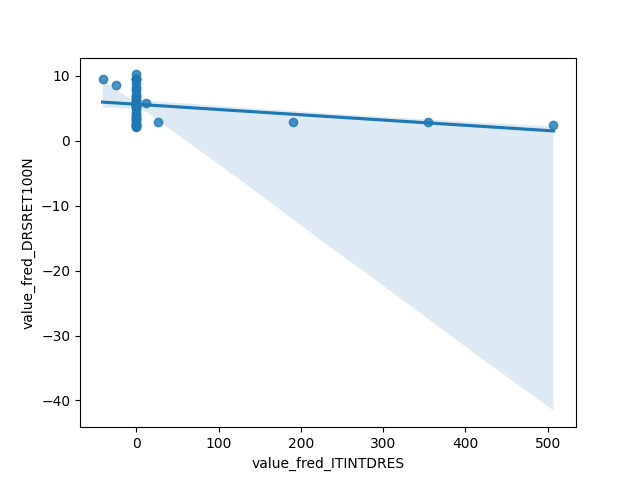
\includegraphics[scale = 0.9]{plots/plot_2026-08-05.png}
\caption{Raw Regression Plot for 2026-08-05}
\end{figure}
\newpage
\subsection{Detrended Regression}
\noindent Regresses the residuals of each series after removing its own linear time trend, so a shared trend can no longer drive the result on its own. A relationship that stays significant here is better evidence of a genuine link between the two series.

\begin{center}
\begin{tabular}{lclc}
\toprule
\textbf{Dep. Variable:}                    & value\_fred\_DRSRET100N\_detrended & \textbf{  R-squared:         } &     0.021   \\
\textbf{Model:}                            &                OLS                 & \textbf{  Adj. R-squared:    } &    -0.002   \\
\textbf{Method:}                           &           Least Squares            & \textbf{  F-statistic:       } &    0.9112   \\
\textbf{Date:}                             &          Wed, 05 Aug 2026          & \textbf{  Prob (F-statistic):} &    0.345    \\
\textbf{Time:}                             &              13:32:38              & \textbf{  Log-Likelihood:    } &   -87.537   \\
\textbf{No. Observations:}                 &                   44               & \textbf{  AIC:               } &     179.1   \\
\textbf{Df Residuals:}                     &                   42               & \textbf{  BIC:               } &     182.6   \\
\textbf{Df Model:}                         &                    1               & \textbf{                     } &             \\
\textbf{Covariance Type:}                  &             nonrobust              & \textbf{                     } &             \\
\bottomrule
\end{tabular}
\begin{tabular}{lcccccc}
                                           & \textbf{coef} & \textbf{std err} & \textbf{t} & \textbf{P$> |$t$|$} & \textbf{[0.025} & \textbf{0.975]}  \\
\midrule
\textbf{const}                             &   -5.314e-13  &        0.273     & -1.95e-12  &         1.000        &       -0.551    &        0.551     \\
\textbf{value\_fred\_ITINTDRES\_detrended} &      -0.0029  &        0.003     &    -0.955  &         0.345        &       -0.009    &        0.003     \\
\bottomrule
\end{tabular}
\begin{tabular}{lclc}
\textbf{Omnibus:}       &  3.670 & \textbf{  Durbin-Watson:     } &    0.127  \\
\textbf{Prob(Omnibus):} &  0.160 & \textbf{  Jarque-Bera (JB):  } &    3.038  \\
\textbf{Skew:}          &  0.532 & \textbf{  Prob(JB):          } &    0.219  \\
\textbf{Kurtosis:}      &  2.275 & \textbf{  Cond. No.          } &     90.8  \\
\bottomrule
\end{tabular}
%\caption{OLS Regression Results}
\end{center}

Notes: \newline
 [1] Standard Errors assume that the covariance matrix of the errors is correctly specified.

\begin{figure}
\centering
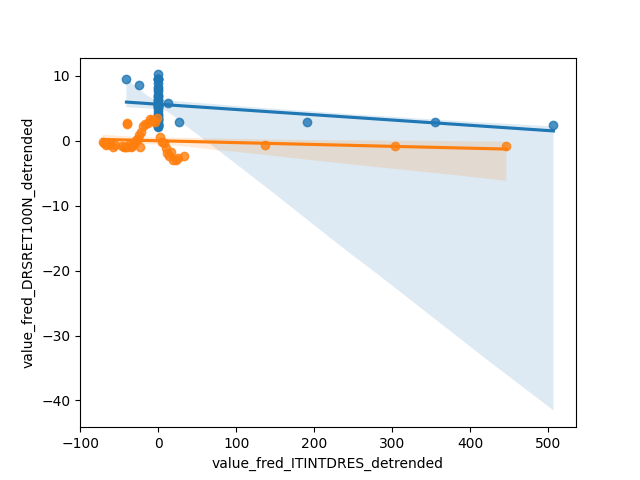
\includegraphics[scale = 0.9]{plots/plot_2026-08-05_detrended.png}
\caption{Detrended Regression Plot for 2026-08-05}
\end{figure}
\newpage
